
\documentclass[a4paper,10pt]{report}
\usepackage{blindtext} % for dummy texts
\usepackage[T1]{fontenc}
\usepackage[table]{xcolor}
\usepackage{titlesec}
\usepackage{graphicx}
%\usepackage[inkscapepath=../assets/svg]{svg}
\usepackage{amsmath}
\usepackage{amsthm}
\usepackage{amssymb}
\usepackage{mathtools}
\usepackage{fancyvrb}
\usepackage[english]{babel}
\usepackage{csquotes}
\usepackage{hyperref}
\usepackage{adjustbox,lipsum}
\hypersetup{
   colorlinks=true,
   linkcolor=blue,
   urlcolor=cyan
}
\usepackage{tikz}
\usepackage{amssymb}
\usepackage[sc]{mathpazo}
\linespread{1.05}
\usepackage{microtype}
\usepackage{breqn}
\usepackage{caption}
\usepackage{subcaption}
\usepackage[
   backend=bibtex,%
   bibencoding=utf8,%
   language=english,%
   style=numeric-comp,%
   sorting=nyt,%
   maxbibnames=10,%
   natbib=true%
]{biblatex}
\addbibresource{references.bib}
\usepackage{siunitx}
\usepackage{booktabs}
\usepackage{longtable}
\usepackage{geometry}
\usepackage{multirow}
\graphicspath{ {../assets/img/} }

\newgeometry{hmargin={30mm,30mm}}

% Set TOC depth and sections numbering
\setcounter{tocdepth}{3}
\setcounter{secnumdepth}{3}

% Remove chapters head and reduce spacing
\titleformat{\chapter}[hang]{\Large\bfseries}{\thechapter \hspace{2ex}}{0pt}{\Large}
\titlespacing{\chapter}{0cm}{0cm}{0.5cm}
\usepackage[parfill]{parskip}

% Make quotes italic
\renewcommand{\mkbegdispquote}[2]{\itshape}

% Change texttt line breaks
\renewcommand{\texttt}[1]{%
  \begingroup
  \ttfamily
  \begingroup\lccode`~=`.\lowercase{\endgroup\def~}{.\discretionary{}{}{}}%
  \catcode`/=\active\catcode`[=\active\catcode`.=\active
  \scantokens{#1\noexpand}%
  \endgroup
}

\titlespacing{\chapter}{0pt}{20pt}{0pt}


\begin{document}
\frenchspacing



%----------------------------------------------------------------------------------------
%	TITLE SECTION
%----------------------------------------------------------------------------------------
\title{
  {{\large{\textsc{Alma Mater Studiorum $\cdot$ University of Bologna}}}}
  \rule{\textwidth}{0.4pt}\vspace{3mm}
  \textbf{Project 4 - Food Recognition\footnote{The code for the project is publicly available on \href{https://github.com/gmurro/FoodRecognition}{GitHub}}}
  \begin{figure}[!htb]
    \centering
    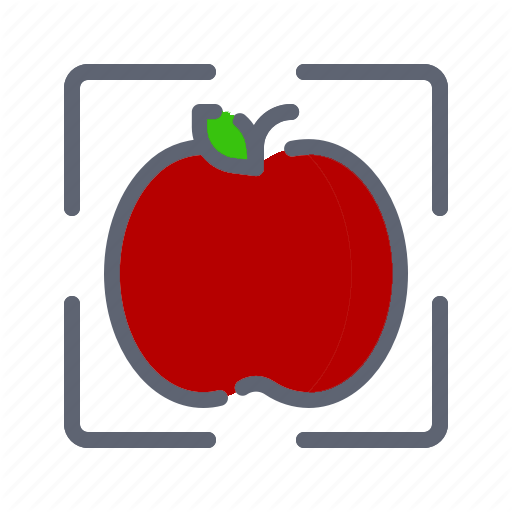
\includegraphics[width = 100pt]{icon}
  \end{figure} \\
   91250 - Deep Learning
}

\author{ Giuseppe Murro (\href{mailto:giuseppe.murro@studio.unibo.it}{giuseppe.murro@studio.unibo.it}) \\ Salvatore Pisciotta (\href{mailto:salvatore.pisciotta2@studio.unibo.it}{salvatore.pisciotta2@studio.unibo.it})}
\date{\today}
\maketitle
\newpage
\tableofcontents
\setcounter{tocdepth}{1}
%\listoffigures
%\listoftables
\newpage
%----------------------------------------------------------------------------------------



%----------------------------------------------------------------------------------------
%	INTRODUCTION
%----------------------------------------------------------------------------------------
{\let\clearpage\relax\par \chapter{Introduction}\label{chap:introduction}
Recognizing food from images is an extremely useful tool for a variety of use cases. In particular, it would allow people to track their food intake by simply taking a picture of what they consume. Current nutritional monitoring apps use traditional methods for food recognition, with algorithms based on classification. However, such applications are either semi-automatic, which identifies a
group of possible types of food and requires user interaction.
Image-based food recognition has in the past few years made substantial progress thanks to advances in deep learning. But food recognition remains a difficult problem for a variety of reasons.
%----------------------------------------------------------------------------------------



%----------------------------------------------------------------------------------------
%	CHAPTER 2: Problem definition
%----------------------------------------------------------------------------------------
\chapter{Problem}\label{chap:problem}

\section{Description}\label{sec:section-21}
The goal of this project is to train models which can look at images of food items and detect, in the form of image segmentation, the individual food element. The categories of food to recognize are limited to a given a set of categories decided in function of the dataset used. Once that the neural networks used for the food recognition are trained, prediction on test set of images are made and based on them results are computed using some metrics.


\section{Dataset}\label{sec:section-22}
The dataset used for this project is the dataset provided in the Food Recognition challenge proposed by AICrowd \cite{aicrowd}, in particular the dataset is divided in  training set, val set and test set. The dataset is structured as follow:
\begin{itemize}
    \item \emph{Training Set} of 24120 (as RGB images) food images with their corresponding 39328 annotations in MS-COCO format
    \item \emph{Validation Set} of 1269 (as RGB images) food images with their corresponding 2053 annotations in MS-COCO format
    \item \emph{Test Set} where there are provided the same images as the validation set
\end{itemize}
}


%----------------------------------------------------------------------------------------


%----------------------------------------------------------------------------------------
%	CHAPTER 3: Approach
%----------------------------------------------------------------------------------------
\chapter{Approach}\label{chap:chapter-3}

\section{Preprocessing}\label{sec:section-31}
The first preprocessing operation that has been done is the filtering of the categories that model can detect. It has been necessary to do this since the dataset provide lots of categories and images that, if totally used for training a neural network, would require high computation capability. So, it has been agreed to reduce the number of categories down to 16 and in the same way include only those images of the dataset where these classes are present. Following this idea, for the training it has been created a subset of the entire dataset. The categories that has been taken into account are the most present in the dataset considering the entire distribution of categories that is shown in \ref{fig:{dataset_dist}}:

\begin{figure}[h]
  \center
  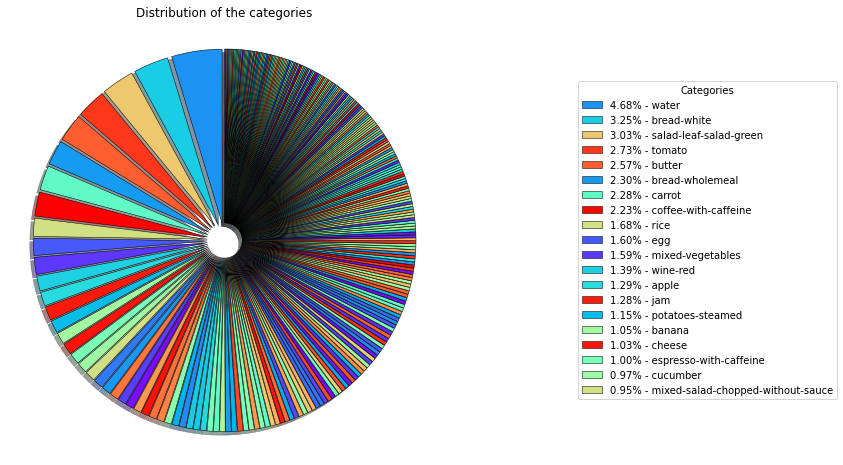
\includegraphics[width=0.9\linewidth]{assets/img/dataset_distr.png}
  \caption{Pie chart of the distribution of the categories in the dataset}
  \label{fig:{dataset_dist}}
\end{figure}


As we can see the most frequent categories are:
\begin{enumerate}
    \item \emph{water}
    \item \emph{bread-white}
    \item \emph{salad-leaf-salad-green}
    \item \emph{tomato}
    \item \emph{butter}
    \item \emph{carrot}
    \item \emph{coffee-with-caffeine}
    \item \emph{rice}
    \item \emph{egg}
    \item \emph{mixed-vegetables}
    \item \emph{wine-red}
    \item \emph{apple}
    \item \emph{jam}
    \item \emph{potatoes-steamed}
    \item \emph{banana}
    \item \emph{cheese}
\end{enumerate}

These first 16 classes are the selected ones. Including the \emph{background} class, the total number of categories has become 17.
The dataset has been reduced as follow:
\begin{itemize}
    \item \emph{Train set} : from 24120 images to 10819
    \item \emph{Val set}: from 1269 images to 554
    \item \emph{Test set} : from 1269 images to 554
    \item \emph{Total number of annotations in the training set} : from 39328 annotations to 12869
\end{itemize}


\section{Multichannel masks}\label{sec:section-32}
One of the most important choice to do was to decide how to encode the classes present in the images into the corresponding masks. In particular how to represent the different categories that are inside a single image. The selected technique in order to deal with multiclass image is the so-called multichannel masks associated to every image. This technique consists in creating an output channel for each of the possible classes. Where every single channel represent the target by one-hot encoding the class labels. For apply this method it has been used Numpy matrices putting in the last dimension the encoding of every channel.
A representation of this methodology is represented in \ref{fig:{multimask}}:

\begin{figure}[h]
  \center
  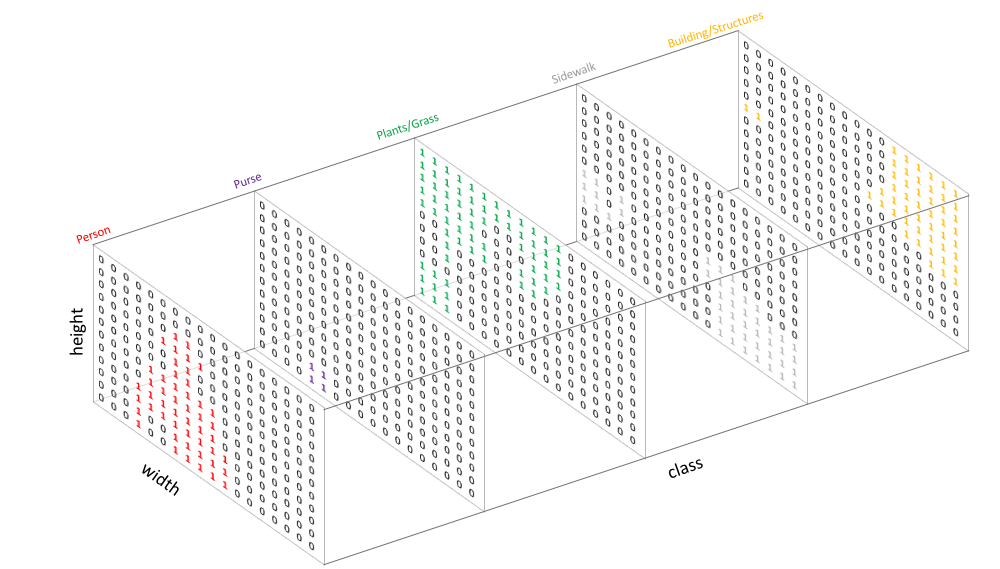
\includegraphics[width=0.7\linewidth]{assets/img/multimask.png}
  \caption{Example of multichannel mask with one-hot encoded channels for every category}
  \label{fig:{multimask}}
\end{figure}


\section{Data Generator}\label{sec:section-33}
Even if the dataset used for the training is a subset of the original, it is still too big to be loaded into memory at once and you could run out of RAM.
That is the reason why there was the need to find other ways to do that task efficiently.
A good solution is using of \textit{data generators}, that can read images on the the fly when they will be used for training.

Keras allow to create custom data generators inheriting the properties of \emph{keras.utils.Sequence} in order to leverage nice functionalities such as multiprocessing.
Every single \emph{Sequence} implements the methods:
\begin{itemize}
    \item \emph{__getitem__}, that should return one batch of data \emph{(X,y)}
    \item \emph{__len__}, that should return the number of batches per epoch
    \item \emph{on_epoch_end}, which is triggered once at the very beginning as well as at the end of each epoch. It allow to shuffle the dataset to make some randomness at each epoch
\end{itemize}

Each image and mask is processed by the \textit{DataGenerator} using pycocotools API \cite{cocoapi} to convert annotations in multichannel masks and then they are resized to \textit{128x128}. So the shape of the input and output data in each batch become:
\begin{itemize}
    \item \emph{X.shape = [batch_size, 128, 128, 3]}
    \item \emph{y.shape = [batch_size, 128, 128, 17]}
\end{itemize}
The channel 0 on the output represent the background and it is composed by all 1s where the category
mask is absent. The example of how the input and output are formed is shown in figure \ref{fig:example_masks}.

\begin{figure}[h]
    \centering
    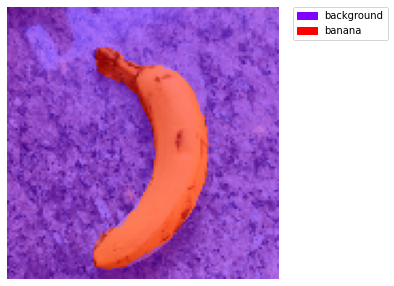
\includegraphics[width=0.45\textwidth]{assets/img/banana.png}
    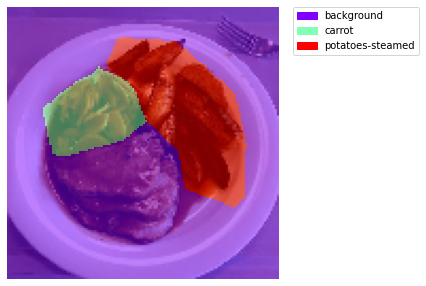
\includegraphics[width=0.45\textwidth]{assets/img/potatoes.png}
    \caption{Examples of image masks}
    \label{fig:example_masks}
\end{figure}

\section{Data Augmentation}\label{sec:section-34}
Data augmentation is the application of a wide range of techniques used to generate "new" training samples \cite{augmentation}. In order to apply augmentation to the project it was implemented a generative function that creates a batch of augmented images and masks for the passed set of images and their correspondent masks.
The term batch of augmented images it is referred to a data generator that instead of simply taking images from the dataset it applies some modifications on them. These modifications are applied to the images using the Keras ImageDataGenerator class that, passing some parameters, applies the same transformations to the image and the correspondent mask.
The used transformations are:
\begin{itemize}
    \item \emph{Rotation} (rotation range = 5\textdegree)
    \item \emph{Width shift} (width shift range = \text{1\%})
    \item \emph{Height shift} (height shift range = \text{1\%})
    \item \emph{Shear shift} (shear range = \text{1\%})
    \item \emph{Horizontal flip} (zoom range = \text{from 90\% to 100\%})
    \item \emph{Vertical flip}
    \item \emph{Zoom}
\end{itemize}

The figure \ref{fig:example_aug} shows an example of how augmentation is computed on the images of figure \ref{fig:example_masks}.

\begin{figure}[h]
    \centering
    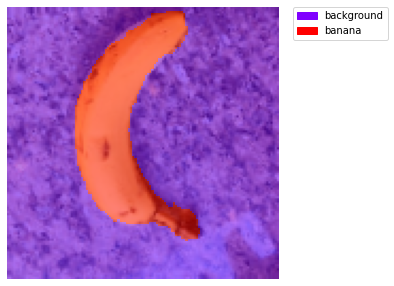
\includegraphics[width=0.45\textwidth]{assets/img/banana_aug.png}
    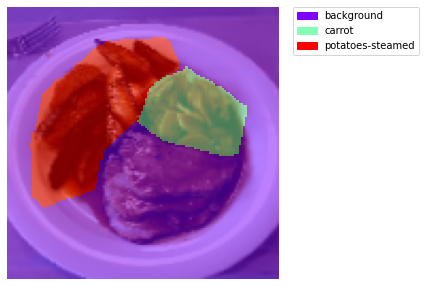
\includegraphics[width=0.45\textwidth]{assets/img/potatoes_aug.png}
    \caption{Examples of augmentation}
    \label{fig:example_aug}
\end{figure}

\section{Activation functions}\label{sec:section-35}
The activation function of the last layer in a convolutional neural network is the one in charge of classifying the category each pixel belongs to. 
Since the output should be a probability, softmax
and sigmoid are the principal candidates. 

For \textit{multi-label classification problem}, where there is more than one "right answer" (the outputs are not mutually exclusive), it is usually better to use a sigmoid function on each raw output independently. Indeed, the sigmoid allows to have high probability for all classes, for only some of them, or for none of them.

Instead for \textit{multi-class classification problem}, where there is only one "right answer" (the outputs are mutually exclusive), it is usually better to use a softmax function. Indeed, the softmax enforces that the sum of the probabilities of output classes are equal to one, so in order to increase the probability of a particular class, the model must correspondingly decrease the probability of at least one of the other classes.

Upon an inspection of the provided dataset, it has been noticed that overlapping of masks is present in the images, for this reason it has been favored an output with sigmoid.

\section{Loss function}\label{sec:section-36}
Semantic segmentation models usually use a simple categorical cross-entropy loss function during training. However, sometimes slightly more advanced loss functions allow to get the granular information of an image.
In particular the paper of Jadon S. \cite{loss-segmentation} discusses the conditions to determine which loss function might be useful in a given scenario and she classifies loss functions for segmentation into 2 macro categories: distribution based and region based.
The most interesting ones per each category, analyzing the dataset used in this project, are \textit{focal loss} and \textit{dice loss}.

\subsection{Focal loss}\label{subsec:subsection-361}
The \textit{focal loss} is a distribution based loss that works better with highly-imbalanced dataset.
It is an improvement to the standard cross-entropy criterion. This is done by changing its shape such that the loss assigned to well-classified examples is down-weighted. In this loss function, the cross-entropy loss is scaled with the scaling factors decaying at zero as the confidence in the correct classes increases. The scaling factor automatically down weights the contribution of easy examples at training time and focuses on the hard ones.
The definition given by Lin T. et al. \cite{focal_loss} is: 
\begin{center}
    $FL(p_t) = -\alpha_t(1 - p_t)^\gamma \cdot \log(p_t)$
\end{center}
where $\gamma \in (0,5]$ and $\alpha$ is a weighting factor $\in [0,1]$

\subsection{Dice loss}\label{subsec:subsection-362}
The Dice coefficient is a widely used metric in computer
vision community to compute the similarity between two
images. This measure ranges from 0 to 1 where a Dice coefficient of 1 denotes perfect and complete overlap. The Dice coefficient was originally developed for binary data, and it can be calculated as: 
\begin{center}
    $Dice = \frac{{2\left| {A \cap B} \right|}}{{\left| A \right| + \left| B \right|}}$
\end{center}

where $\left| {A \cap B} \right|$ represents the common elements between sets A and B, and $\left| A \right|$ represents the number of elements in set A (and likewise for set B).
In order to formulate a loss function which can be minimized, it can be simply used $1 - Dice$. This loss function is known as \textit{soft Dice loss}. It is a region based loss and as Dice coefficient is non-convex in nature, so it has been modified to make it more tractable. It is called in this way because it directly uses the predicted probabilities instead of thresholding and converting them into a binary mask (see figure \ref{fig:dice_loss}). 

\begin{figure}[h]
    \centering
    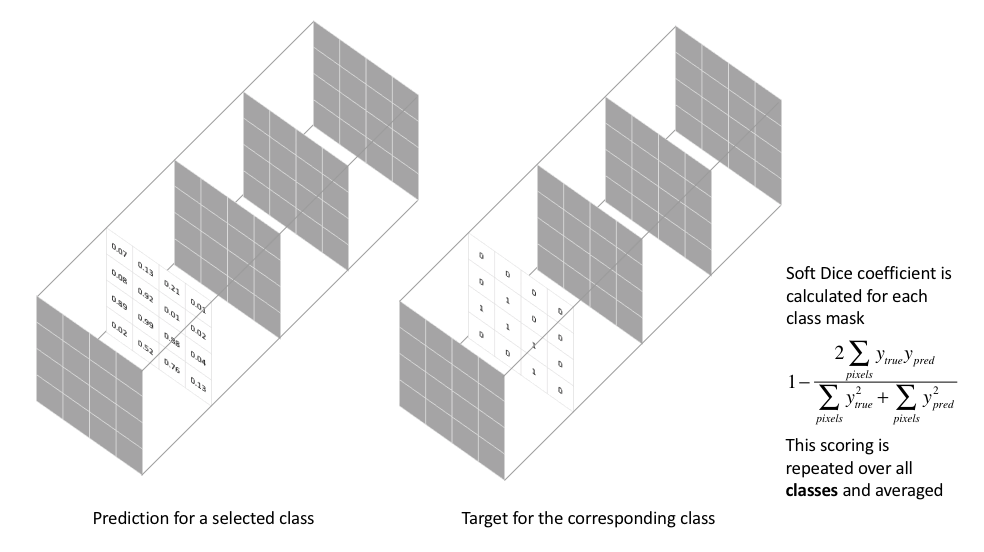
\includegraphics[width=0.65\textwidth]{assets/img/dice_loss.png}
    \caption{How Dice loss is computed \cite{semantic-segmentation}}
    \label{fig:dice_loss}
\end{figure}

\subsection{Combo Loss}\label{subsec:subsection-363}
The final loss that has been used in this project is a sum of \textit{dice loss} and \textit{focal loss}. It attempts to combine their strengths and mitigate their drawbacks.

\section{Class weights}\label{sec:section-37}
Semantic segmentation datasets can be highly imbalanced meaning that particular class pixels can be present more inside images than that of other classes. Since segmentation problems can be treated as per-pixel classification problems we can deal with imbalance problem by weighing the loss function to account for this. It's a simple and elegant way to deal with this problem. 
The class weights are computed for each category with the following formula \cite{class_weights}:
\begin{center}
    $w(y) = \frac{n\_samples}{n\_classes \cdot counts(y)}$
\end{center}

%----------------------------------------------------------------------------------------


%----------------------------------------------------------------------------------------
%	CHAPTER 4: Model
%----------------------------------------------------------------------------------------
\chapter{Model}\label{chap:chapter-4}

\section{Architectures}\label{sec:section-41}
The chosen architecture for the problem resolution is U-Net, originally developed for segmenting biomedical images. When visualized its architecture looks like the letter U and hence the name U-Net. Its architecture is made up of two parts, the left part (the contracting path) and the right part (the expansive path). The purpose of the contracting path is to capture context, while the role of the expansive path is to aid in precise localization.
Two U-Net like models have been investigated in order to compare their effectiveness on food recognition task.

\subsection{Basic U-Net}\label{subsec:subsection-411}
The first architecture is based on the original one proposed by Olaf Ronneberger et al. \cite{unet}, and it is is illustrated in figure \ref{fig:basic-unet}. 

The contracting path starts from an image of size \emph{(128x128x3)} and follows the typical architecture of a convolutional network. It consists of four repeated application of two 3x3 convolutions (unpadded convolutions), each followed by a rectified linear unit (ReLU) and a 2x2 max pooling operation with stride 2 for downsampling. 
At each downsampling step the number of feature
channels are doubled (starting from 32 up to 512), while the spatial dimensions is cutted by half (starting from 128 up to 8). The bottleneck uses two 3X3 convolutional layers to produce an internal encoding of the input image. 

The expansion section consists of several expansion blocks with each block passing the input to two 3X3 convolutional layers and a 2x2 “up-convolution” that halves the number of feature channels. It also includes a concatenation with the correspondingly cropped feature map from the contracting path. The cropping is necessary due to the loss of border pixels in
every convolution. In the end, 1X1 convolutional layer is used to produce 17 feature maps as same as the number of categories which are desired in the output.

\begin{figure}[h]
    \centering
    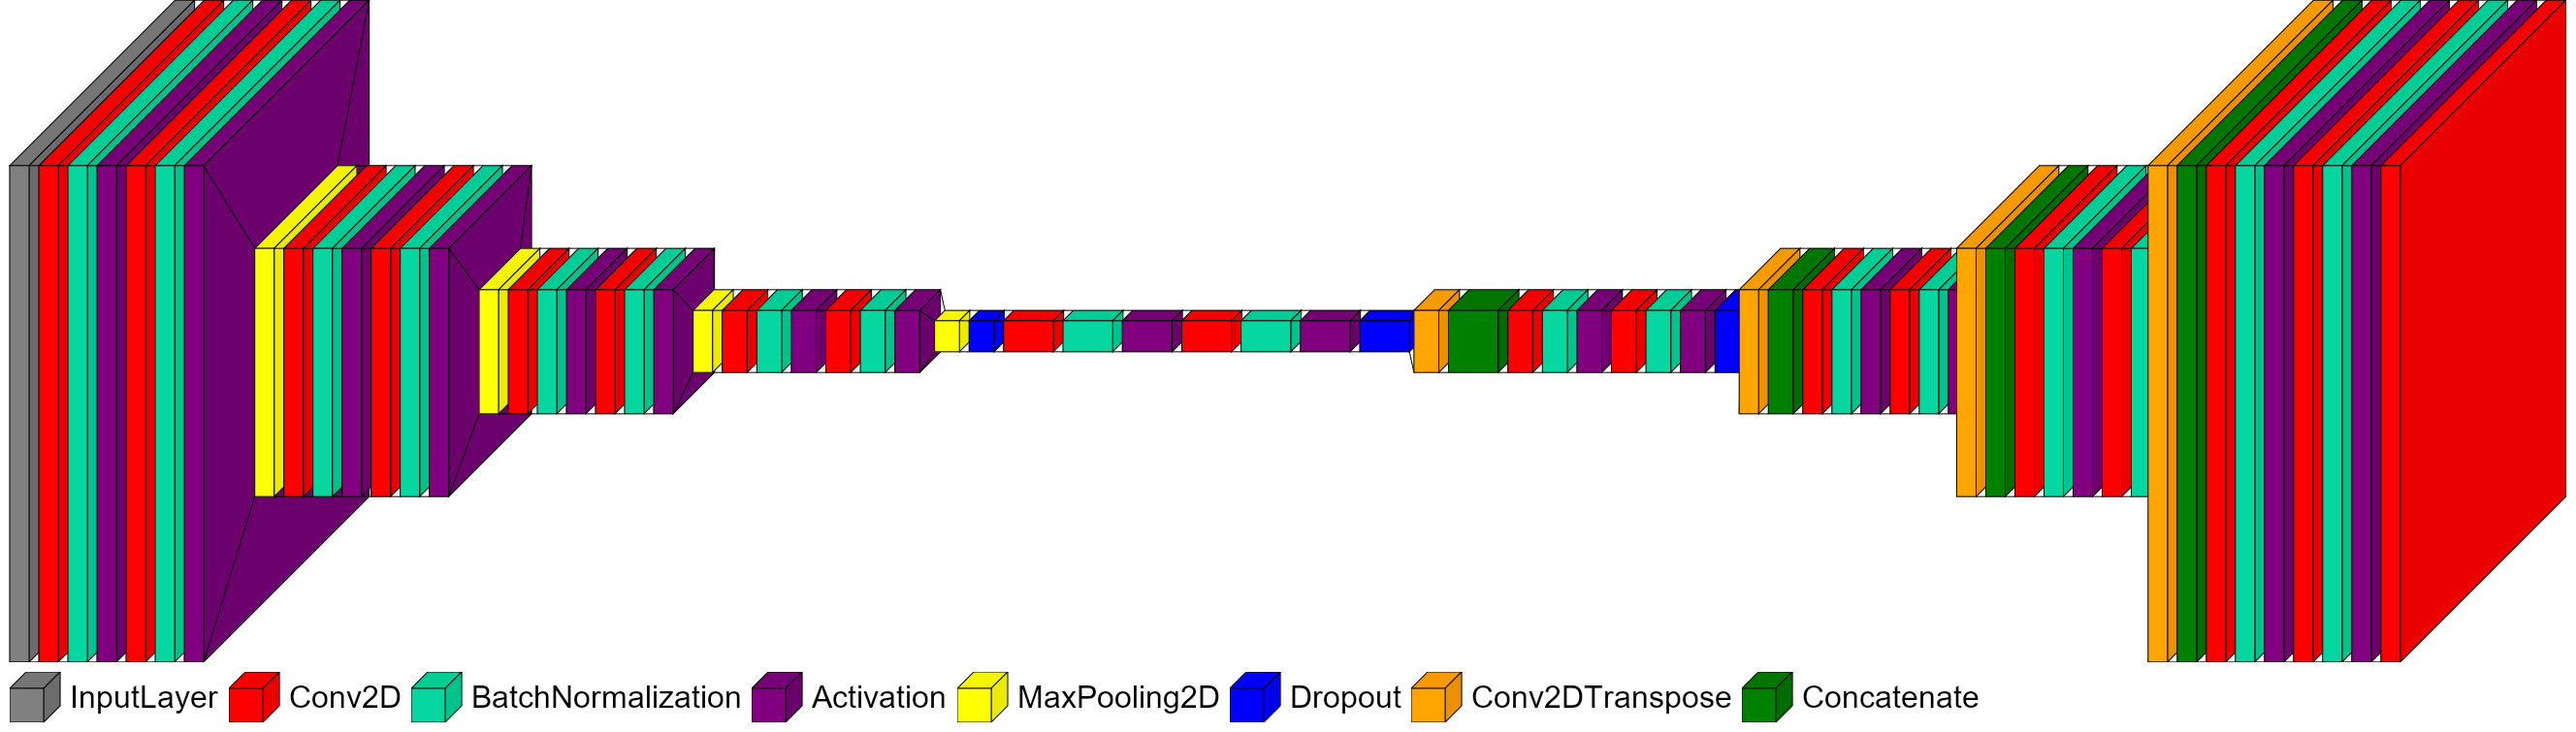
\includegraphics[width=0.8\textwidth]{assets/img/unet.png}
    \caption{Architecture of the basic U-Net}
    \label{fig:basic-unet}
\end{figure}

\subsection{Eff U-Net}\label{subsec:subsection-412}
The second architecture is inspired by Baheti B. et al. \cite{effunet} which propose a novel approach for semantic segmentation that use EfficientNet as feature extractor in encoder and UNet as decoder. 

The EfficientNet, as proposed in \cite{effnet}, consists of the compound coefficient which studied model scaling and adjusted the depth, width, and the resolution of the network for better performance.
A new baseline architecture called EfficientNetB0 was designed initially and it is scaled up to generate family of EfficientNet by compound scaling method. Powered by this approach, there are eight variants of the EfficientNets, namely EfficientNetB0 to EfficientNetB7. As illustrated in figure \ref{fig:effnet_compare} a good compromise between number of parameters (in order to avoid a too heavy training) and accuracy is EfficientNetB5 and it is used as encoder in the implemented model. 


\begin{figure}[h]
  \centering\begin{minipage}[b]{0.37\textwidth}
    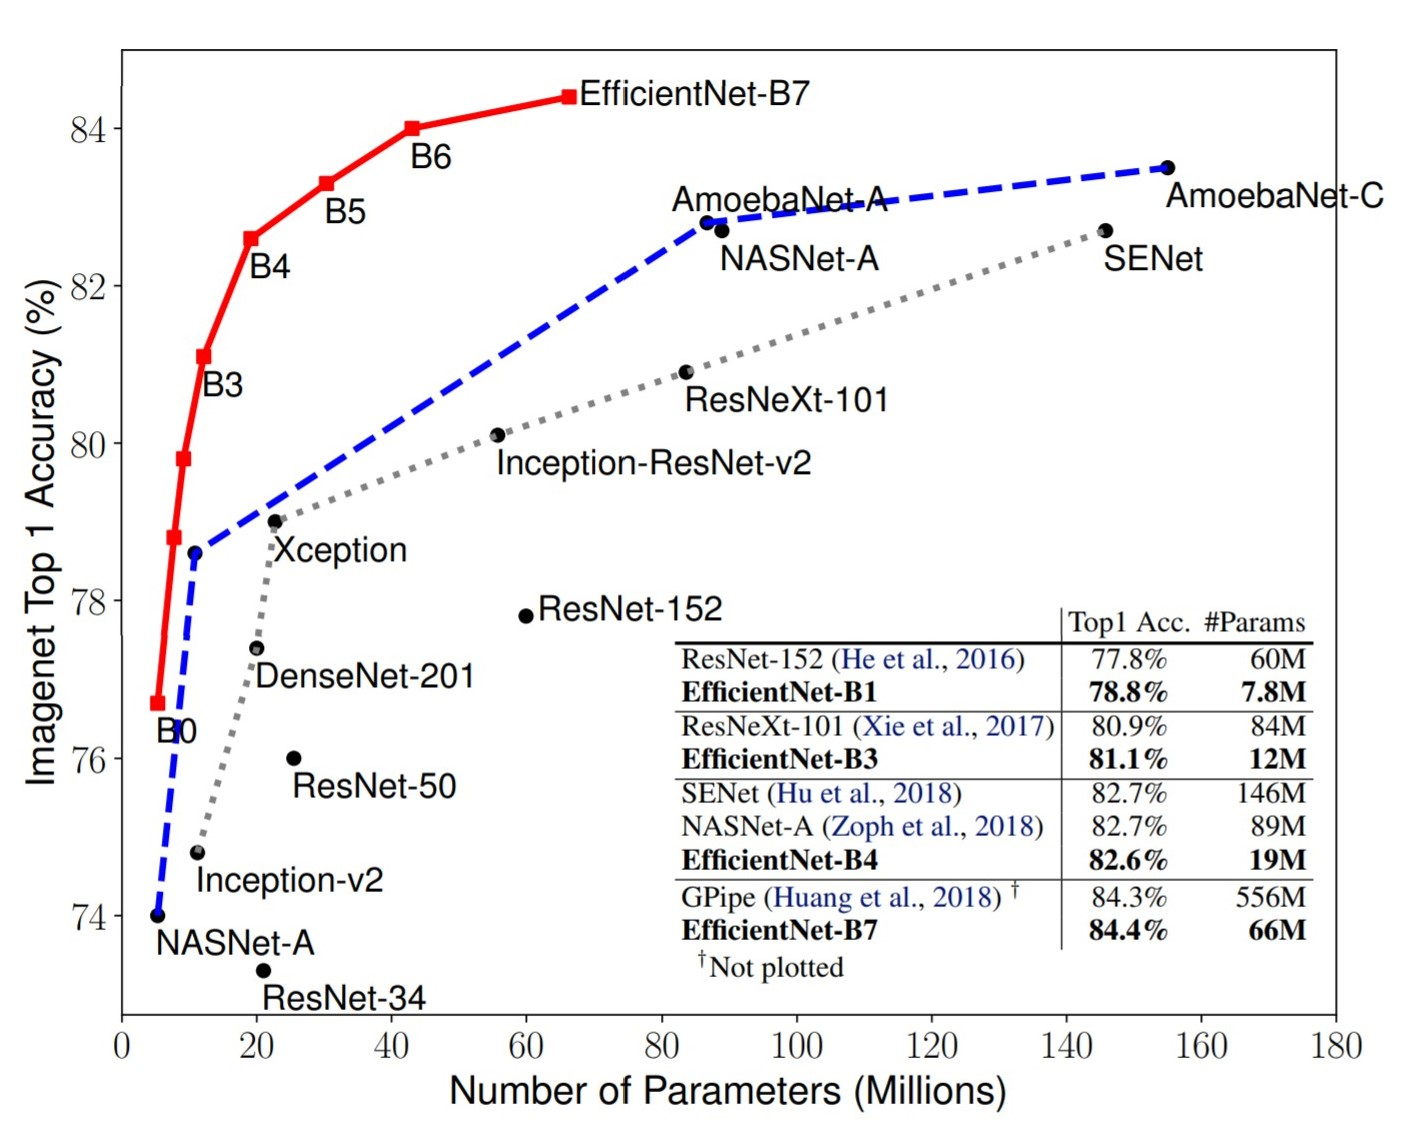
\includegraphics[width=\textwidth]{assets/img/effnet_compare.png}
\caption{Eff-Nets comparison \cite{effnet}}
\label{fig:effnet_compare}
  \end{minipage}
  \hfill\begin{minipage}[b]{0.62\textwidth}
    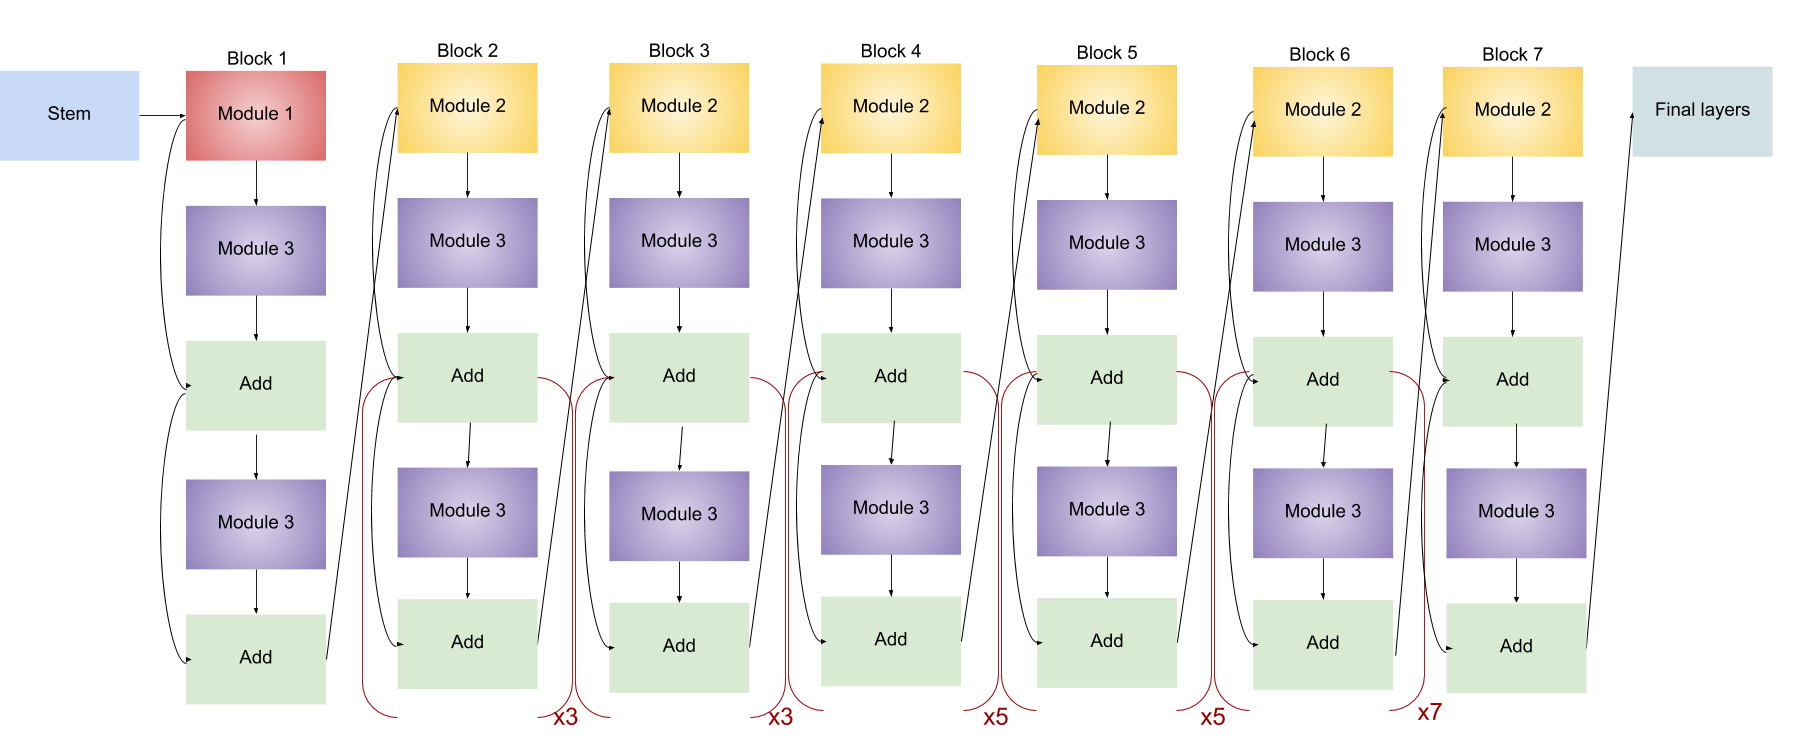
\includegraphics[width=\textwidth]{assets/img/effunetB5.png}
    \caption{Architecture of EfficientNetB5 \cite{effnetB5}}
\label{fig:effnetb5}
  \end{minipage}
\end{figure}

The structure of EfficientNetB5, illustrated in figure \ref{fig:effnetb5}, is composed by 7 building blocks of several mobile inverted bottleneck convolutions (MBConv) with squeeze and excitation optimization. 
The final Eff U-Net model appear like in figure \ref{fig:effunet} where the decoder is similar to the original U-Net and as usual blocks from the contracting path are connected with the corresponding layers in the expansion path.

\begin{figure}[h]
    \centering
    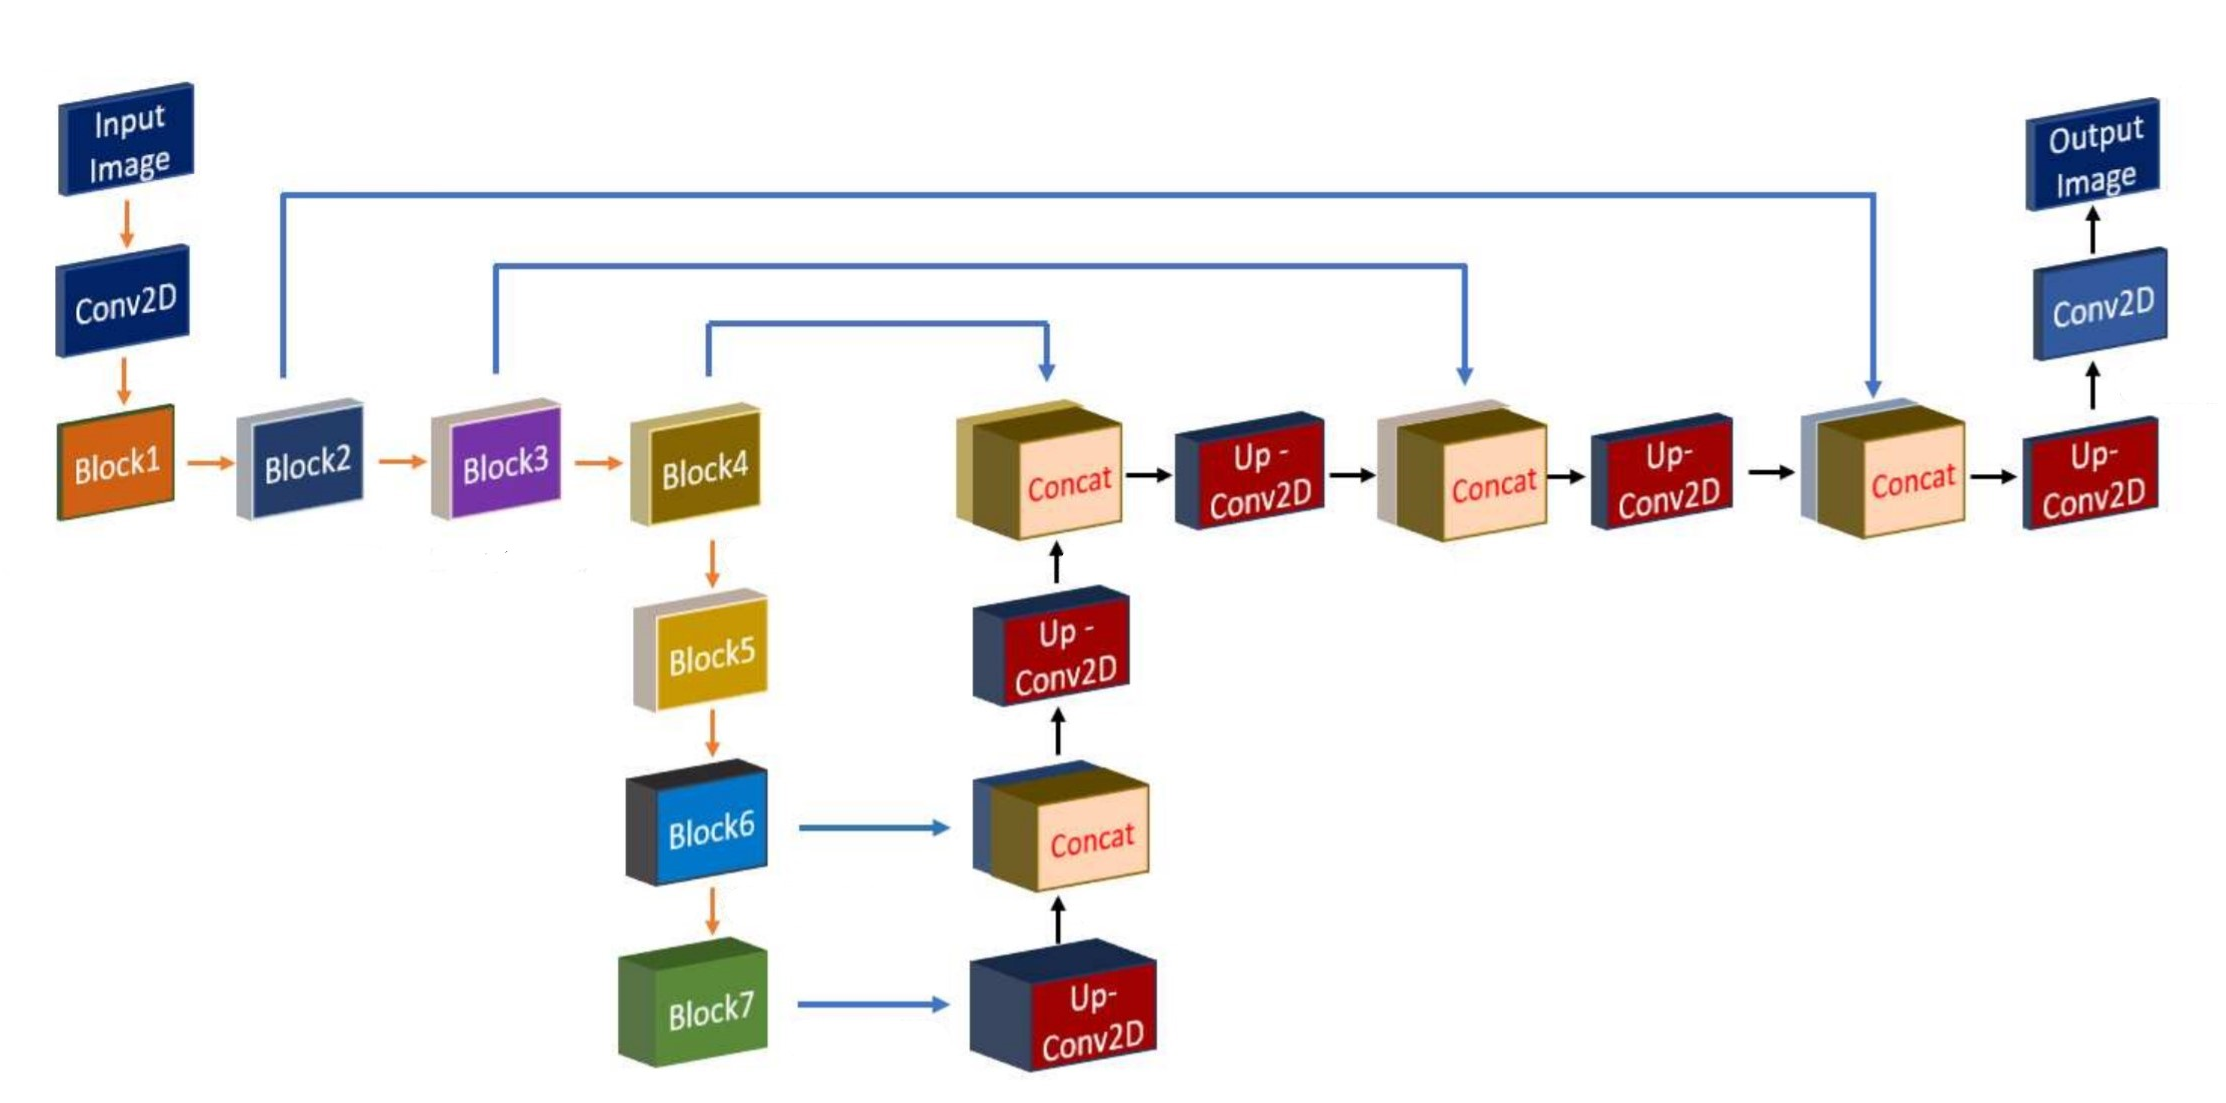
\includegraphics[width=0.70\textwidth]{assets/img/effunet.png}
    \caption{Architecture of Eff U-Net}
    \label{fig:effunet}
\end{figure}


\section{Training}\label{sec:section-42}
\subsection{Hardware used}\label{subsec:subsection-421}
Training is a highly demanding task in terms of both computing and memory usage, so it is important to use properly the available resources. 
For that purpose, it is used a machine with those specifications:
\begin{itemize}
    \item Intel® Core™ i7-10750H (6 core)
    \item RAM DDR4 16 GB
    \item NVIDIA® GeForce RTX™ 2060 6 GB
    \item Windows 10 Home 64
\end{itemize}

The training is done using \textit{Keras} with \textit{Tensorflow 2.4.1} as backend since it support GPU computation, which speeds up the training some orders of magnitude.

\subsection{Experiments}\label{subsec:subsection-422}
During the training phase, several sessions have been scheduled in order to test the combination of different hyper-parameters.
The common hyper-parameters fixed for each attempt are:
\begin{itemize}
    \item batch size: 64
    \item epochs: 80
    \item optimizer: Adam with learning rate = 0.001
    \item class weights used for weighting the loss function
    \item metrics: IOUScore, Precision, Recall, FScore (provided by \emph{segmentation_models} library \cite{segmentation-models})
\end{itemize}

The most promising models were the ones illustrated in table \ref{table:models} where have been alternated the losses \textit{Dice Loss (DL) +  Binary Focal Loss (BFL)} and \textit{Dice Loss (DL) +  Categorical Focal Loss (CFL)} and also an attempt without augmentation has been done.

\begin{table}[h]
\center
  \begin{tabular}{|c|c|c|c|c|c|c|}
  \hline
    \multirow{2}{*}{} & \multicolumn{6}{c|}{\textbf{Models description}}  \\ \hline 
                        & \textbf{Architecture} & \textbf{Activation} & \textbf{Loss}& \textbf{Epochs} & \textbf{Trainable Params} & \textbf{Augmentation} \\ \hline
    \textbf{Model A}   & Basic U-Net & Sigmoid & BFL + DL & $80$ & $7.766.513$ & Yes \\ \hline
    \textbf{Model B}      & Basic U-Net & Sigmoid & BFL + DL & $80$ & $7.766.513$ & No \\ \hline
    \textbf{Model C}       & Basic U-Net & Softmax & CFL + DL & $80$ & $7.766.513$ & Yes  \\ \hline
    \textbf{Model D} & Eff U-Net & Sigmoid & BFL + DL & $80$ & $17.293.649$ & Yes \\ \hline
  \end{tabular}
  \caption{Description of models}
  \label{table:models}
\end{table}


For the Eff U-Net training it has been applied the \textit{transfer learning}, a popular method that allows to build accurate models in a timesaving way reusing models trained on a different but somehow similar problem.
Indeed, instead of starting the learning process from scratch it relies on pre-trained weights based on ImageNet. In this way the convolutional base has been freezed on its original form and it uses pre-trained weights to get feature extraction.
As can be observed from the figure \ref{fig:plot}, the latter model seems to be the best and, thanks to transfer learning, the loss decreases much faster than other models in early epochs.

\begin{figure}[h]
    \centering
    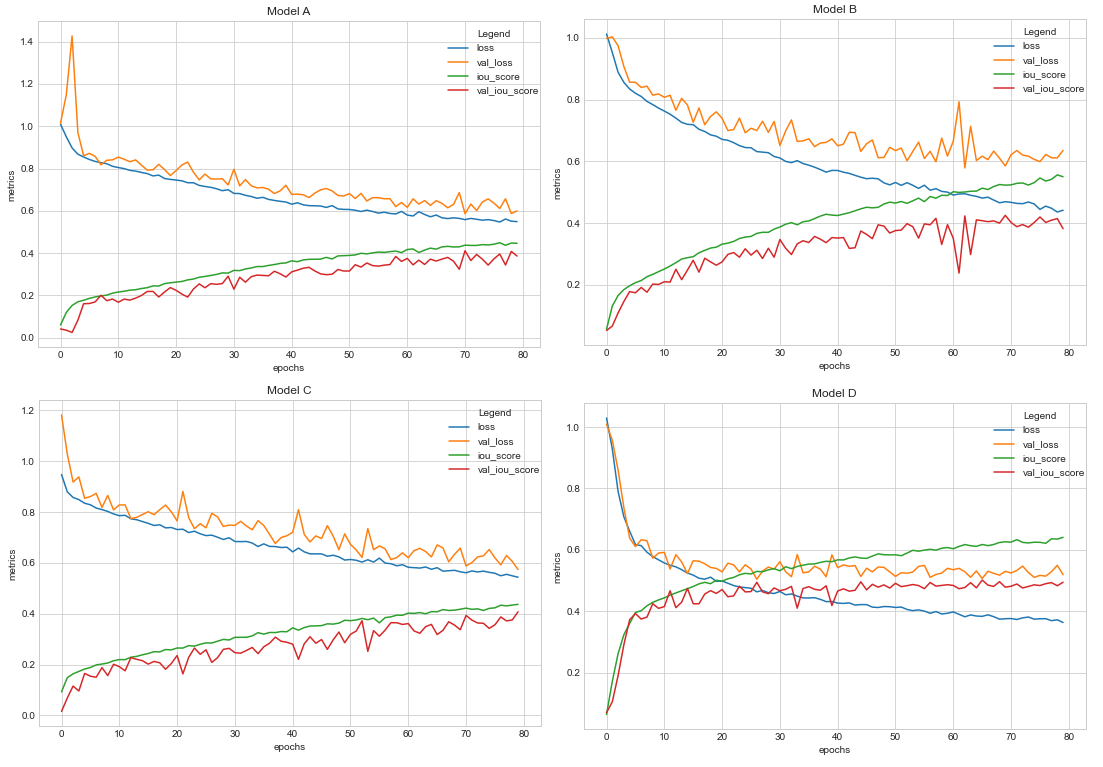
\includegraphics[width=0.98\textwidth]{assets/img/plots.png}
    \caption{History of models during the training}
    \label{fig:plot}
\end{figure}


%----------------------------------------------------------------------------------------


%----------------------------------------------------------------------------------------
%	CHAPTER 5: Evaluation
%----------------------------------------------------------------------------------------
\chapter{Evaluation}\label{chap:chapter-5}

All the predictive masks before the evaluation have been processed by a method that given in input the masks produced by the neural network, where it is associated a probability to each pixel , return a binarized masks where each pixel is 1 or 0 depending if the probability is over a certain threshold. The used threshold value, empirically selected, is 0.4 .

\section{Metrics}\label{sec:section-51}
In order to evaluate results produced by different models' predictions on the test set of images,there were used three metrics that are required by the project to and that are the most used at the state of art \cite{metrics}
\begin{itemize}
    \item \emph{IoU}: Intersection over Union
    \item \emph{Precision}
    \item \emph{Recall}
\end{itemize}

\subsection{IoU}\label{subsec:subsection-511}

The intersection over union \ref{fig:iou}, known also as Jaccard index, is the ratio between the area of overlap and the area of union of the ground truth and prediction, where the overlap can be calculated as the intersection between the two masks.

In the evaluation of the results of prediction the IoU is calculated for every different channel present in the image and the final image IoU is the mean of IoU of every channel.
The final result is the mean of every single image IoU that is called mIoU.


\begin{figure}[h]
  \centering\begin{minipage}[b]{0.37\textwidth}
    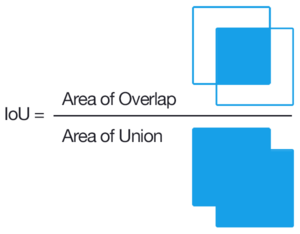
\includegraphics[width=\textwidth]{assets/img/IoU.png}
\caption{Intersection over Union}
\label{fig:iou}
  \end{minipage}
  \hfill\begin{minipage}[b]{0.60\textwidth}
    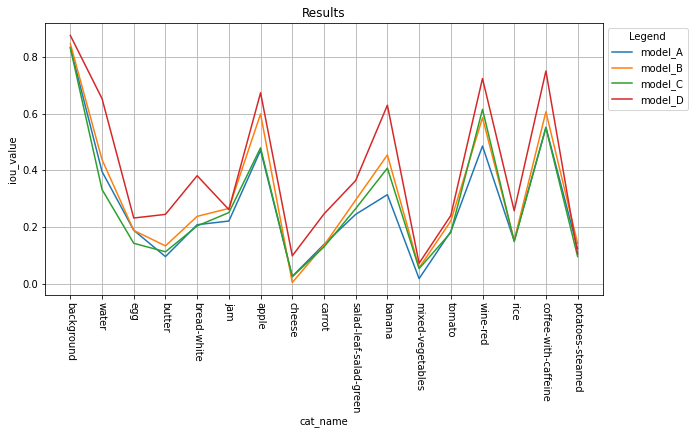
\includegraphics[width=\textwidth]{assets/img/cat_iou.png}
    \caption{IoU values computed by for every category}
\label{fig:cat_iou}
  \end{minipage}
\end{figure}

\clearpage\subsection{Precision}\label{subsec:subsection-512}

The precision effectively describes the purity of our positive detections relative to the ground truth. Precision is calculated as the ratio between true positive and the sum between true positive and false positive results. 


\[Precision = \frac{TP}{TP + FP}\]

In this project it was used the Keras Precision class passing the ground truth mask and the predicted mask.
Simirarly to IoU results also the precision results are computed initially for each single image as the mean of the precision of every class present in the image and then compute the mean of all the images as final precision result computed by the model on the predictions of the test set.

\begin{figure}[h]
    \centering
    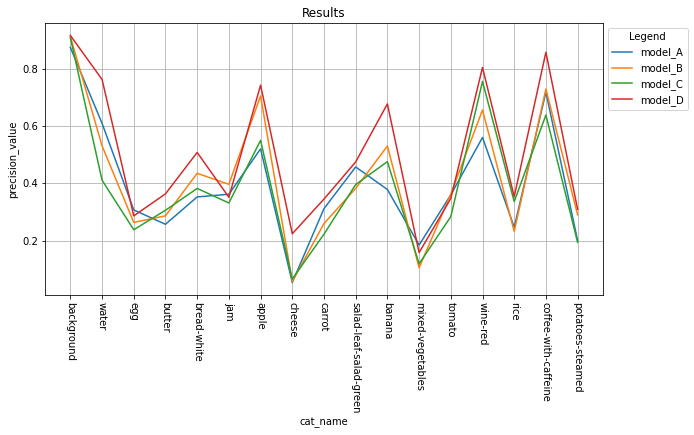
\includegraphics[width=0.7\textwidth]{assets/img/cat_prec.png}
    \caption{Precision values computed by every model for every category}
    \label{fig:cat_prec}
\end{figure}

\clearpage\subsection{Recall}\label{subsec:subsection-513}
The recall describes the completeness of our positive predictions relative to the ground truth. Recall is calculated as the ratio between true positive and the sum between true positive and false negative results. 


\[Recall = \frac{TP}{TP + FN}\]

Also in this case it was used the Keras Recall class passing the ground truth mask and the predicted mask and again, similarly to IoU and precision results, also the recall results are computed initially for each single image as the mean of the recall of every class present in the image and then compute the mean of all the images as final recall result computed by the model on the predictions of the test set.

\begin{figure}[h]
    \centering
    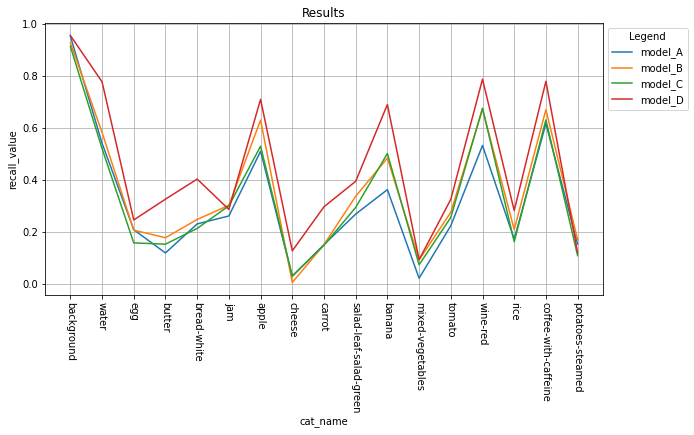
\includegraphics[width=0.7\textwidth]{assets/img/cat_recall.png}
    \caption{Recall values computed by every model for every category}
    \label{fig:cat_recall}
\end{figure}


\clearpage\section{Results}\label{sec:section-52}

The results that can be seen in the table \ref{table:test_results} are the final values of every metric computing the mean of every image values. It is important to say that these results take into account all the classes present in every single image (include the background class). Following some resources it can be seen that there are conflicting opinions on whether or not to take the background class into account in the calculation of the metrics. The final decision was to take into account also the background class following the suggestions of an AICrowd forum discussion about the evaluation criteria \cite{evalcriteria}

\begin{table}[h]
  \center
  \begin{tabular}{|c|c|c|c|}
  \hline
    \multirow{2}{*}{} & \multicolumn{3}{c|}{\textbf{Test}}  \\ \hline                   
                        & \textbf{IoU} & \textbf{Precision} & \textbf{Recall} \\ \hline
    \textbf{Model A}   & $0.488$ & $0.591$ & $0.559$  \\ \hline
    \textbf{Model B}      & $0.525$ & $0.618$ & $0.591$ \\ \hline
    \textbf{Model C}       & $0.455$ & $0.549$ & $0.526$  \\ \hline
    \textbf{Model D} & $0.624$ & $ 0.703$ & $0.688$  \\ \hline
  \end{tabular}
  \caption{Test results of every model}
  \label{table:test_results}
\end{table}


\begin{figure}[h]
    \centering
    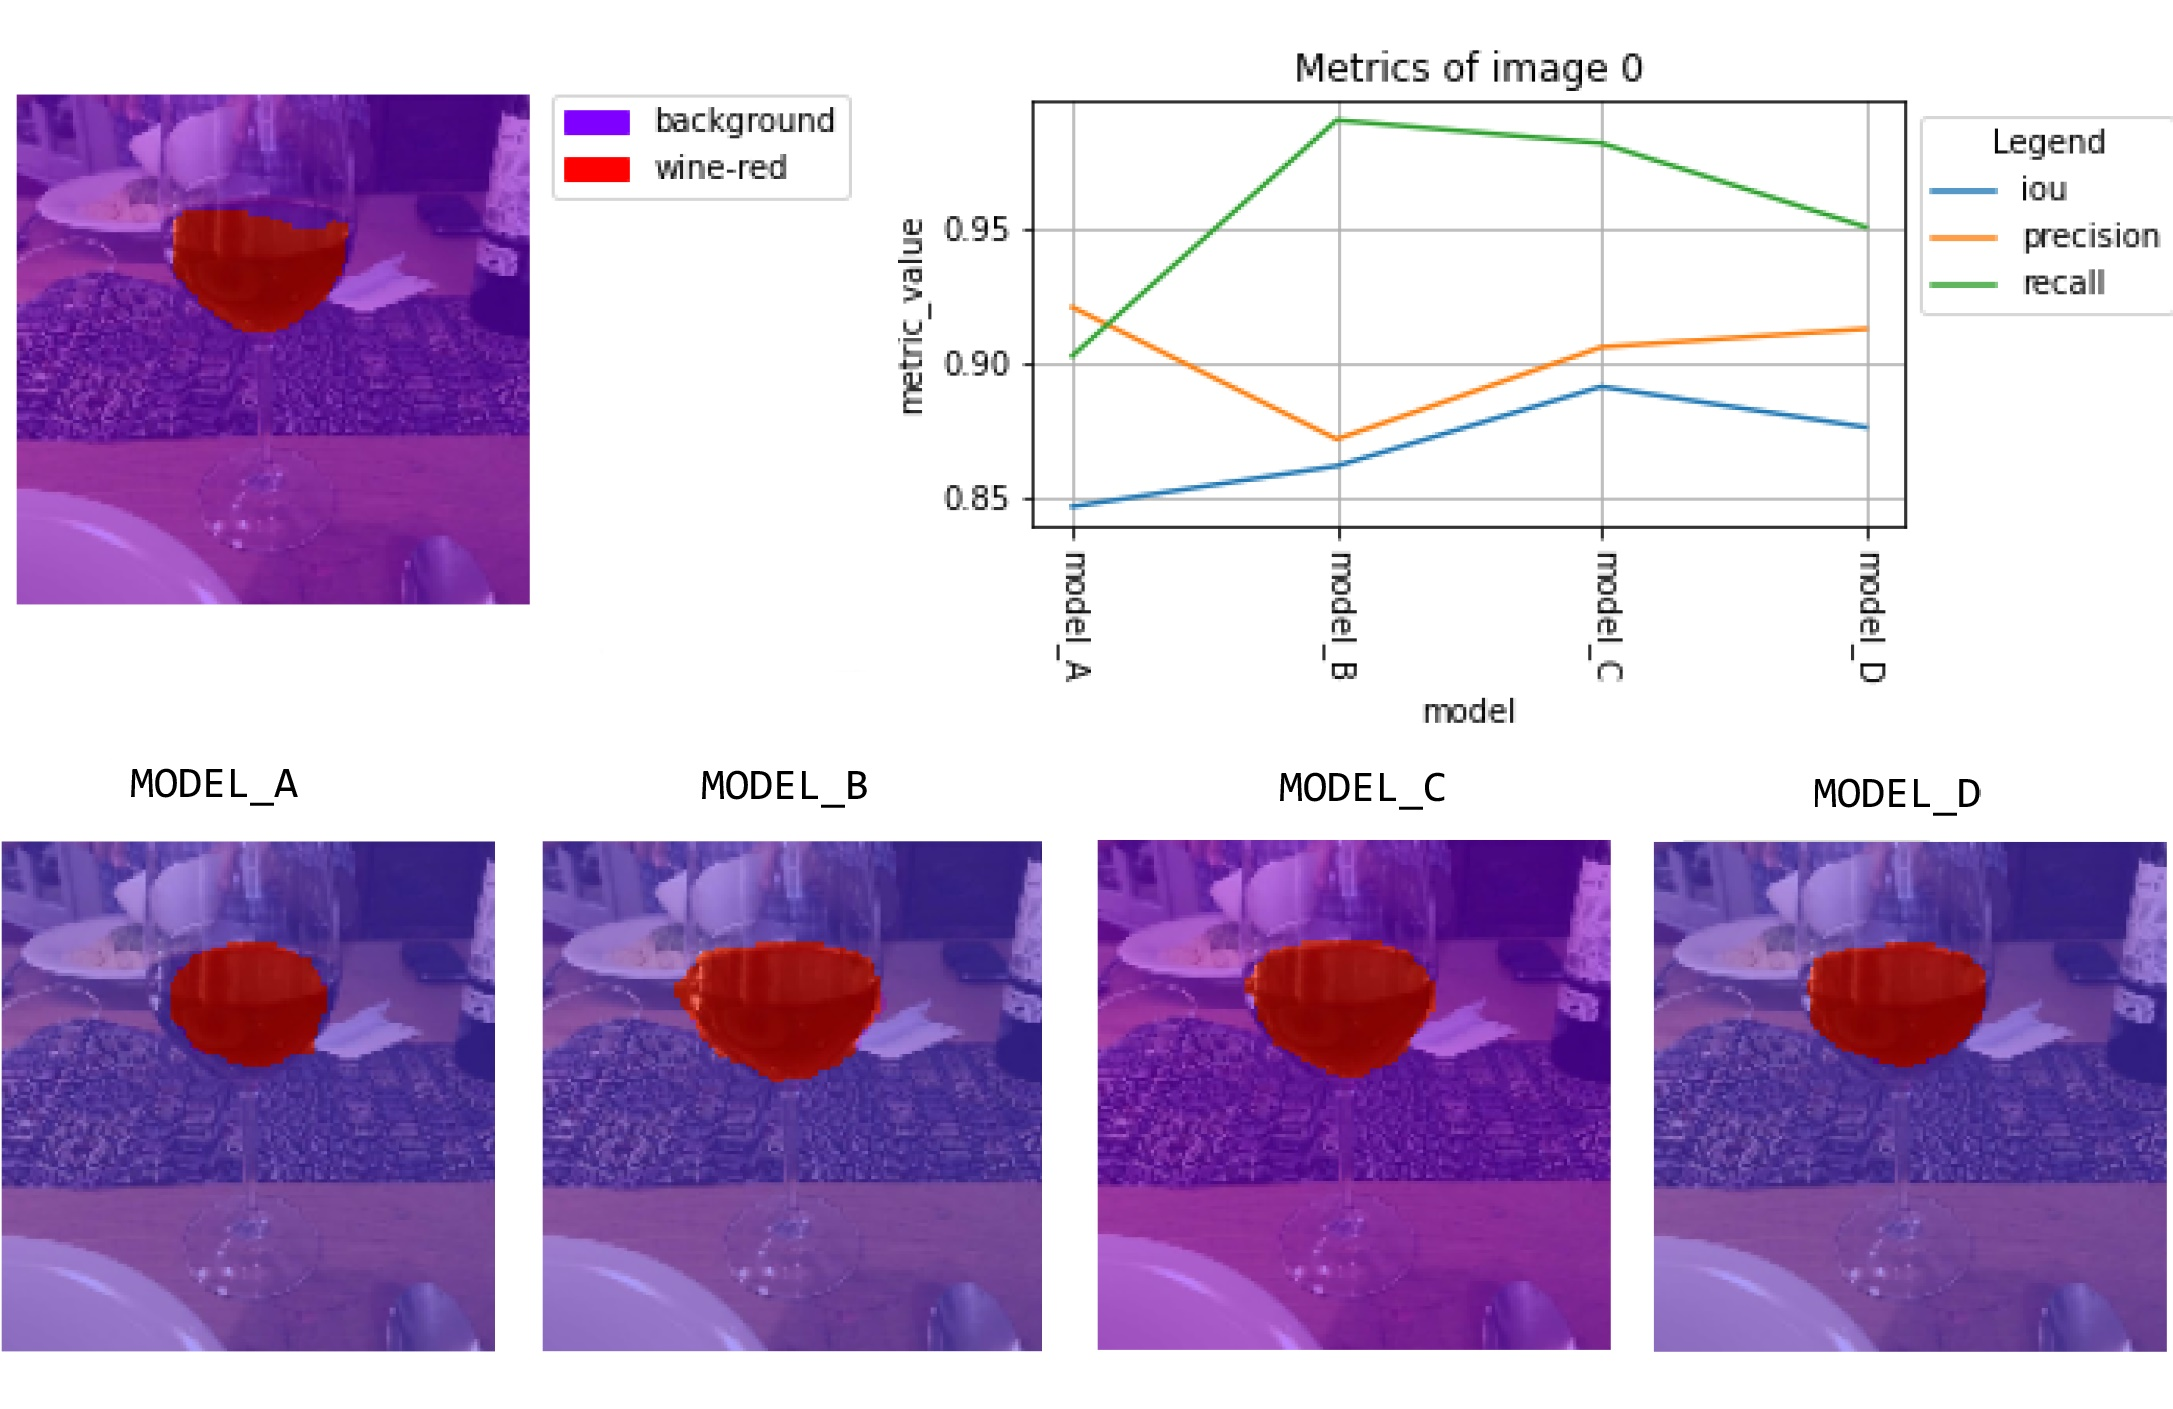
\includegraphics[width=0.7\textwidth]{assets/img/mod_image0.jpg}
    \caption{An example of a well done prediction}
    \label{fig:result0}
\end{figure}

\clearpage 

\begin{figure}[h]
    \centering
    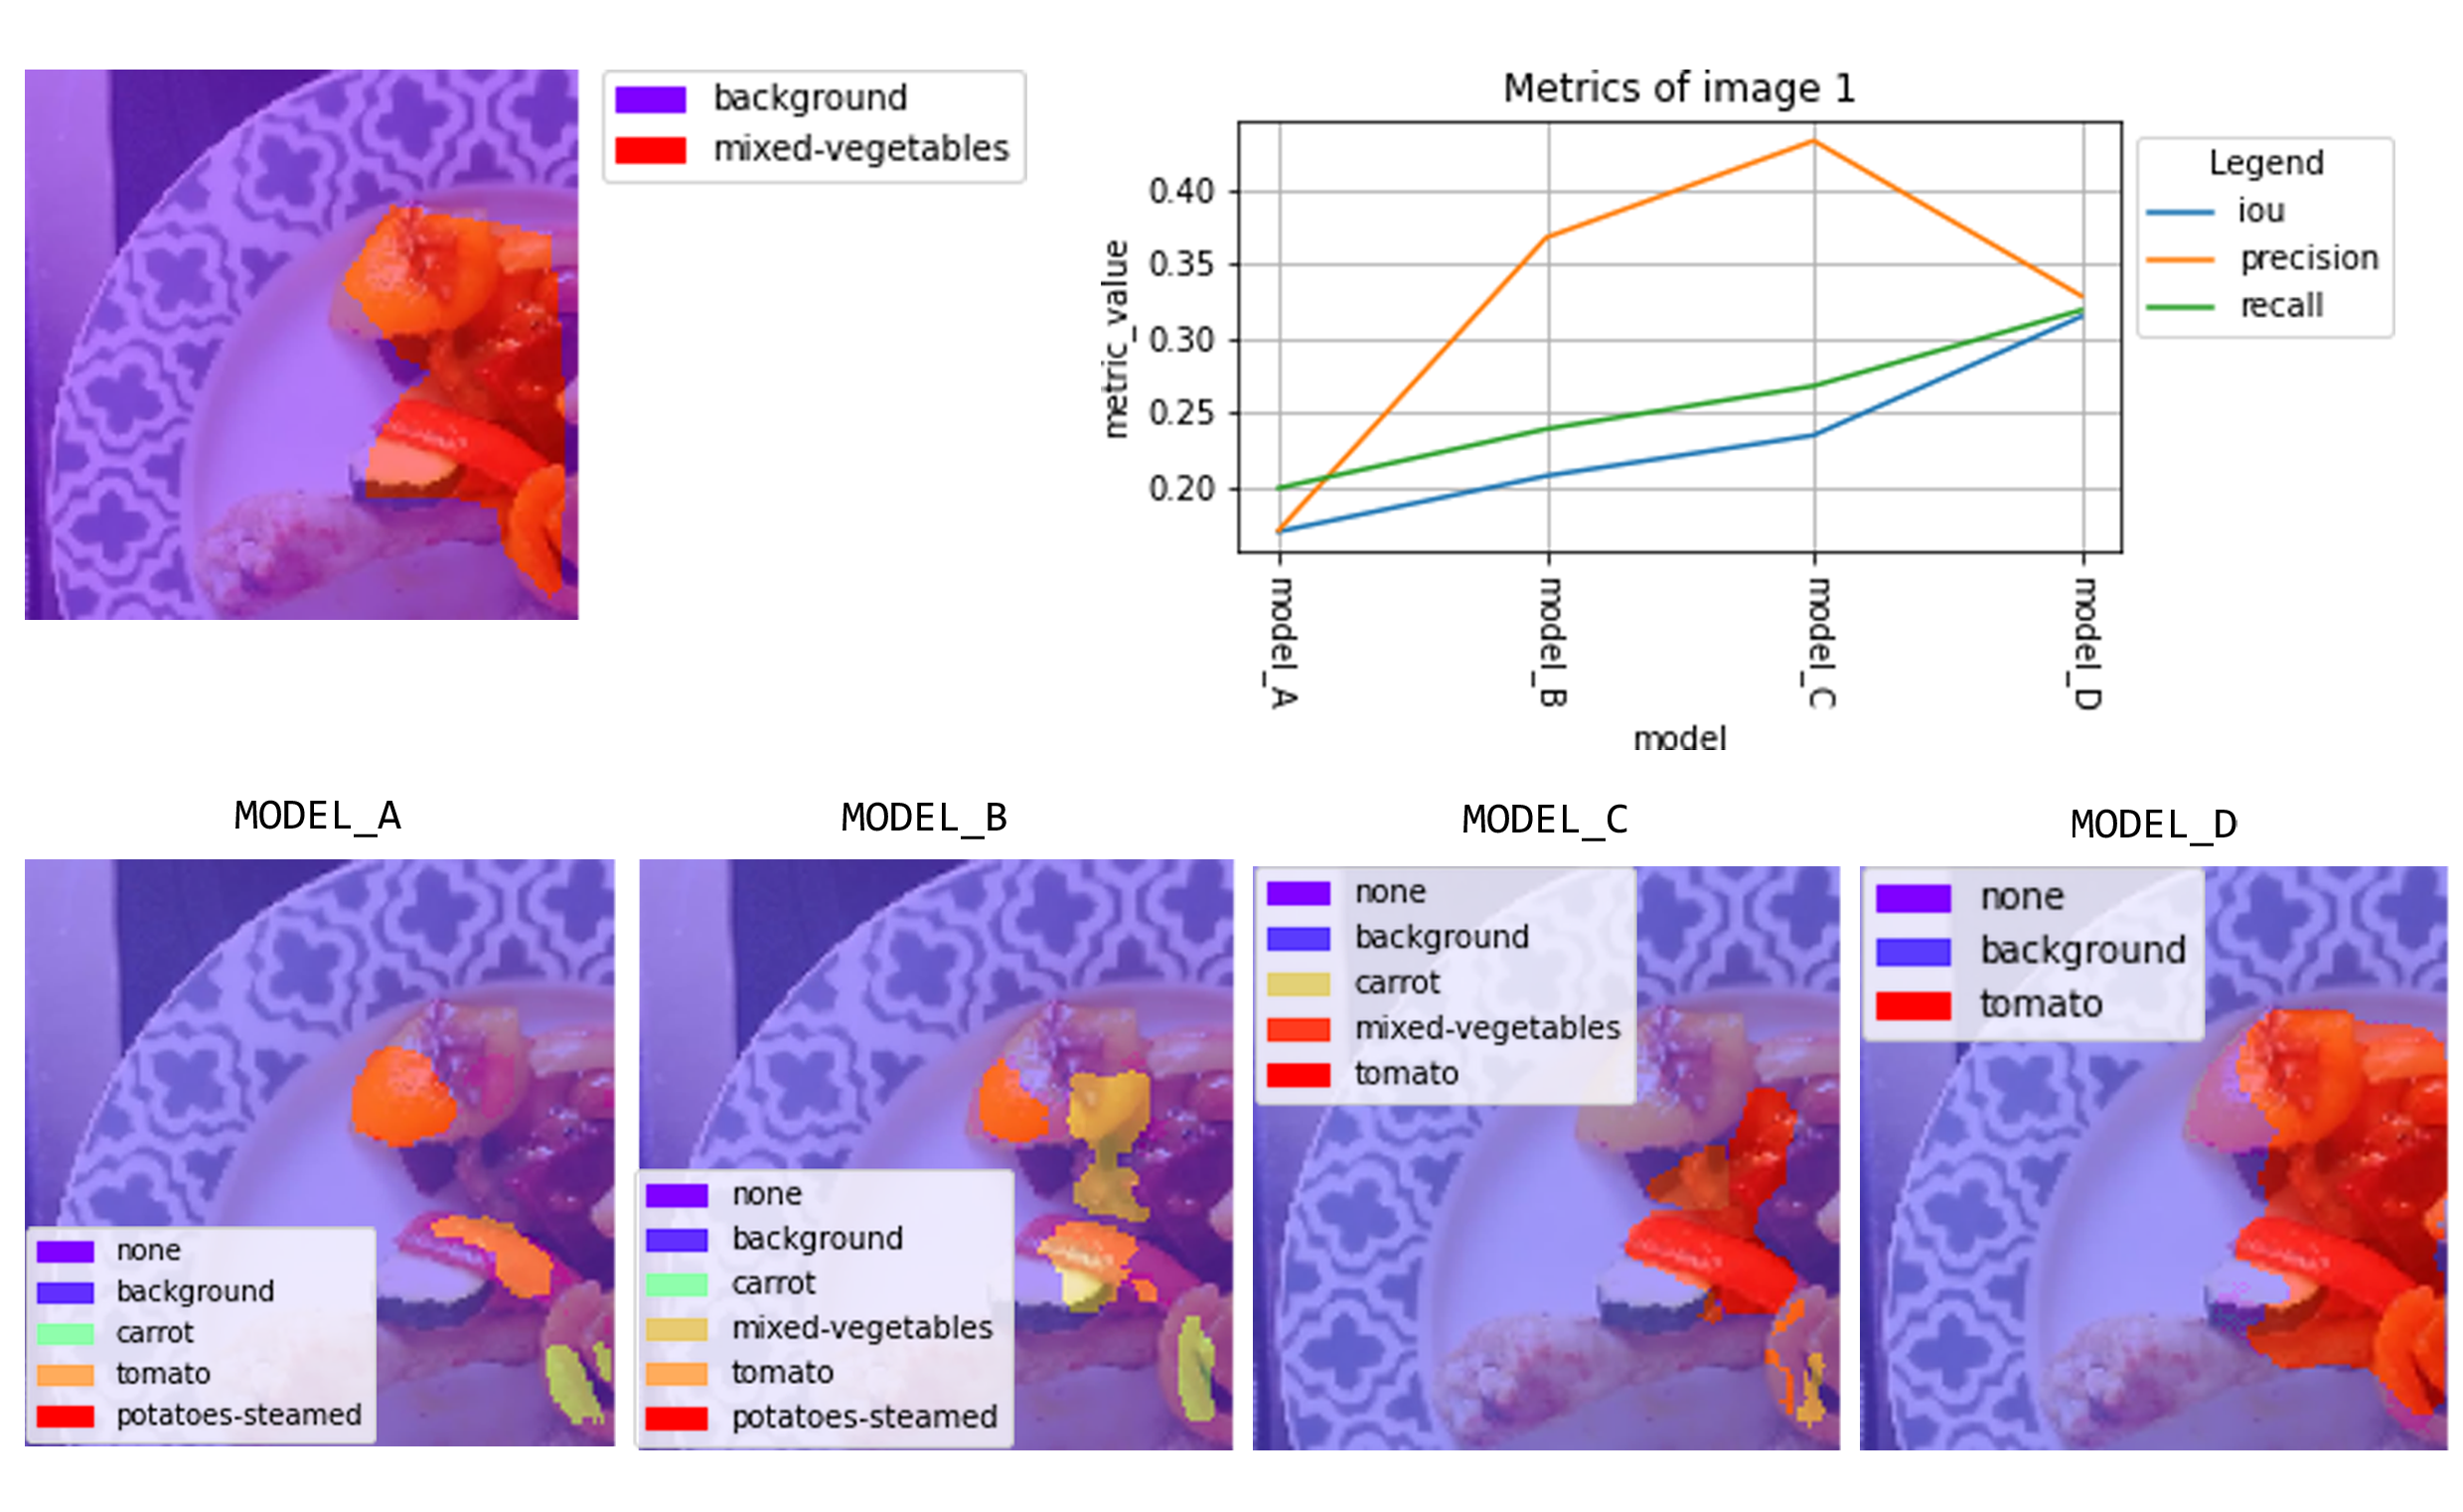
\includegraphics[width=0.7\textwidth]{assets/img/result2.png}
    \caption{An example of a bad done prediction}
    \label{fig:result1}
\end{figure}


%----------------------------------------------------------------------------------------


%----------------------------------------------------------------------------------------
%	CHAPTER 6: Conclusion
%----------------------------------------------------------------------------------------
{\let\clearpage\relax\par \chapter{Conclusions and future works}\label{chap:conclusions}

From the results it is possible to see that the \text{Eff U-Net} is the model that gives the best results with respect to the others considered. In order to improve the work that has been done in this project the first step could be extend the training not only on a subset of the dataset but to the entire dataset. Of course this requires machines with more computational capability than the ones we used for this project. For this reason it is more realistic to improve the project looking for different model that could give better results than the used ones and also try to use different metrics in order to analyze in a more detailed way the results obtained. The last improvement that can be done is on the ground truth annotations, since there are some images where they are not perfectly done o classified a refinement of the annotations can positively influence the final results.
}


%----------------------------------------------------------------------------------------
%	REFERENCES
%----------------------------------------------------------------------------------------
\printbibliography
\end{document}


